% vim: set tw=78 tabstop=4 shiftwidth=4 aw ai:

% \chapter{Measurements of Multimedia Distribution in Peer-to-Peer Networks}
\chapter{Măsurători pentru distribuția multimedia în Peer-to-Peer}
\label{chapter:multimedia-dist}

% A large part of content distribution in the Internet is currently video
% content. Video content means large files, typically movie files of CD or DVD
% size. File size increases if the bitrate or resolution increases. Apart from
% movie files, sites such as YouTube, focusing on small videos that are
% published by average users are attracting millions of users. Content is
% accessed many times and transferred across the Internet.
O mare parte din conținutul distribuit prin Internet este în prezent formată
din conținut video. Acest tip de conținut implică existența unor fișiere mari,
de obicei filme de dimensiunea unui CD sau DVD. Dimensiunea crește odată
cu bitrate-ul sau rezoluția. Pe lângă fișerele ce conțin filme, pagini
precum YouTube, ce se concentrează pe filme scurte, publicate de
utilizatori obișnuiți, atrag milioane de utilizatori. Conținutul este
accesat de multe ori și transferat prin Internet.

% A Peer-to-Peer protocol and BitTorrent, in particular, is one of the most
% adequate solution for distributing large content. Rapid creation of swarms,
% tit-for-tat, rarest-piece first allow BitTorrent to rapidly distributed files
% among peers. When thinking about video content, this mode is known as offline
% playback -- the video file is downloaded and subsequently rendered. Separate
% approaches are to be undertaken for Video-on-Demand and Live Streaming as
% described in Section~\ref{sec:multimedia-dist:video}.
Un protocol Peer-to-Peer și, în particular, BitTorrent, reprezintă una dintre
cele mai potrivite soluții pentru distribuția de conținut de dimensiuni mari.
Crearea rapidă de grupuri, abordarea unui comportament similar (reacția de tip
,,tit-for-tat'') și politica de selecție prioritară a fragmentelor rare permit
BitTorrent să distribuie rapid fișiere între clienți. Când se vorbește despre
conținutul video se face referire la modul de redare offline -- fișierul video
este mai întâi descărcat și abia apoi este redat. Este necesară existența unor
abordări diferite pentru Video-on-Demand și Live Streaming.

% \section{Adding Video Streaming Support in libtorrent}
\section{Adăugarea suportului pentru a reda conținut video în libtorrent}
\label{sec:multimedia-dist:libtorrent}

% libtorrent-rasterbar\footnote{\url{http://www.rasterbar.com/products/libtorrent/}}
% is a popular solution implementing the BitTorrent
% specification\footnote{\url{http://bittorrent.org/beps/bep\_0003.html}} and many of
% its enhancements.  Written in C++ it uses advanced operating system operations
% allowing good performance. It is used by a large number of BitTorrent clients,
% including Deluge, Miro, qBitTorrent, ZipTorrent, LimeWire.

libtorrent-rasterbar\footnote{\url{http://www.rasterbar.com/products/libtorrent/}}
este o soluție binecunoscută ce implementează specificația BitTorrent
\footnote{\url{http://bittorrent.org/beps/bep\_0003.html}} și multe dintre
îmbunătățirile ei. Fiind scrisă în C++, folosește operațiile avansate puse
la dipoziție de sistemul de operare pentru a fi performantă. Este folosită de
un număr mare de clienți de BitTorrent, incluzând Deluge, Miro, qBitTorrent,
ZipTorrent, LimeWire.

% As, from a performance point of view, libtorrent-rasterbar possesses a high
% rank among BitTorrent implementations, it was considered as one of the best
% choices for adding streaming support. libtorrent-rasterbar is used only
% as a classical BitTorrent distribution solution, not as a streaming solution.
% The goal was to provide video on demand (VoD) support by altering the required
% components of the implementation.
Din punct de vedere al performanței, libtorrent-rasterbar ocupă unul dintre
primele locurile printre implementările de BitTorrent și a fost aleasă ca
una dintre cele mai bune opțiuni pentru adăugarea de suport pentru redare
video. libtorrent-rasterbar este folosită doar ca o soluție clasică pentru
distribuirea de conținut prin BitTorrent, dar nu și ca o soluție pentru
redare. Scopul a fost de a pune la dispoziție posibilitatea de redare video la
cerere ("video on demand" - VoD) prin modificarea componentelor necesare din
cadrul implementării existente.

% The piece selection strategy in a typical BitTorrent swarm is based on
% \textit{rarest-first}. This means that each peer tries to acquire the rarest
% piece as the first one ensuring better performance that random packet
% selection~\cite{bt-analysis}\cite{scaling-networks}. An analysis has proven that
% \textit{rarest-first} has the best performance when considering the efficiency
% vs. cost factor.
Strategia de selecție a fragmentului într-un grup BitTorrent tipic este bazată
pe \textit{rarest-first}. Aceasta înseamnă că fiecare client va încerca să
obțină mai întâi cel mai rar fragment, asigurând o performanță mai bună decât
selecția aleatoare a unui fragment~\cite{bt-analysis}\cite{scaling-networks}.
Analiza demonstrează că \textit{rarest-first} are cea mai bună performanță cu
privire la raportul eficiență vs. factorul de cost.

% As a consequence of the particularities of the ``strictly in order'' piece
% selection algorithm, \textit{tit-for-tat} can not be used within a single
% swarm. Peer relations are asymmetrical and a downloader may never serve
% pieces to an uploader. This means that piece requests are non-uniformly
% distributed among the whole swarm. Old peers receive more requests that
% younger peers but may only serve \textbf{U} of them.
Drept consecință a particularităților algoritmului de selecție strict
succesivă (``strictly in order'') a fragmentelor, \textit{tit-for-tat} nu
poate fi utilizat în cadrul unui singur grup. Relațiile între clienți sunt
asimetrice și este posibil ca un client ce descarcă un fragment să nu îl
distribuie niciodată înapoi unuia care îl distribuie. Această înseamnă că
cererile de fragmente nu sunt distribuite uniform în cadrul grupului. Clienții
mai vechi vor primi mai multe cereri decât cei mai noi, dar este posibil să
răspundă la doar o parte dintre ele.

% Presuming, as it usually is the case, a connection that possesses a bandwidth
% capacity higher than the playback rate, an efficient streaming doesn't need to
% employ \textit{strictly in order} piece selection. It only needs a sufficient
% number of packages that allow content playback to happen at a consistent rate,
% while other pieces may be retrieved using other algorithms. A compromise needs
% to be negotiated between sequential progress and download speed, download
% latency and swarm health.
Să presupunem că, așa cum se întâmplă de obicei, o conexiune este caracterizată
de o lățime de bandă mai mare decât rata de redare. Aceasta înseamnă că, pentru
o redare efientă, nu este necesară implementarea algoritmului de selecție
\textit{strictly in order}. Este necesară doar pentru descărcarea unui număr
suficient de pachete care să permită redarea consistentă a conținutului, în
timp ce restul de fragmente pot fi descărcate folosit orice alt algoritm.
Trebuie să se ajungă la un compromis între progresul secvențial și viteza de
descărcare, latența și integritatea grupului.

% In order to achieve that compromise, we define \textit{deadline pieces}. This
% pieces use a deadline specifying when the packet needs to be downloaded. Such
% a packet receives a priority in the pieces selection if it's close to its
% deadline. This way, some of the packets may be downloaded through
% \textit{rarest-first} while others may be downloaded through \textit{strictly
% in order}. Deadlines may be computed by taking into account the media bitrate
% and the number of pieces of the video asset.
Pentru a ajunge la acest compromis, definim fragmente cu termen
(\textit{deadline pieces}). Aceste fragmente folosesc un termen limită pentru
momentul de descărcare al unui pachet. Un astfel de pachet devine prioritar în
timpul selecție fragmentelor dacă termenul lui limită se apropie. Astfel,
unele pachete pot fi descărcate folosind algoritmul \textit{rarest-first},
în timp ce restul pot fi descărcate folosind \textit{strictly in order}.
Termenele limită pot fi calculate ținând cont de biterate-ul mediu și numărul
de fragmente din fișierul video.

% The module implementing the piece selection is a central component in a
% BitTorrent implementation. It is optimized in libtorrent to rapidly find
% rarest pieces. It keeps a list of available pieces, sorted by rarity, and
% equally rare packets are mixed. The \textit{rarest-first} model is the main
% strategy for piece selection. Other models are supported, though their use is
% particular to certain situations.
Modulul ce implementează selecția fragmentelor este o componentă centrală în
implementarea de BitTorrent. Este optimizat în libtorrent pentru găsirea
rapidă a celui mai rar fragment. Menține o listă de fragmente disponibile,
sortate după raritate, iar pachetele care sunt la fel de rare sunt amestecate.
Modelul \textit{rarest-first} este urmat de principala strategie de selecție a
fragmentelor. Și alte modele sunt suportate, deși folosirea lor este limitată
la anumite situații.

% The piece selector allows combining the availability of a given packet with a
% certain piece priority. These parameters determine the criterion used for
% sorting the piece list. Zero priority pieces will never be selected, an option
% used for selective downloading.
Selectorul de fragmente permite combinarea măsurii de disponibilitate a unui
anumit pachet cu o anumită prioritizare a fragmentelor. Acești parametri
determină criteriul folosit pentru sortarea listei de fragmente. Fragmentele
cu prioritate zero nu vor fi niciodată selectate, opțiune folosită pentru
descărcarea selectivă.

% For \textit{strictly in order} implementation, a specialized option dubbed
% \textit{sequential} is added to the piece picker and is checked inside the
% \texttt{piece\_picker::pick\_pieces()} function. A \textit{cursor} variable is
% inserted that stores the index of the last downloaded piece. The interested
% block list is appended the block not already download that can be downloaded
% sequentially from the given peer. New blocks are added in the same manner
% until the requested block limit is reached or no more pieces are available. To
% be remarked that piece request is sequential but not necessarily piece
% delivery.
Pentru implementarea strategiei \textit{strictly in order}, o opțiune
specializată, marcată cu \textit{sequential}, este adăugată selectorului de
fragmente și este verificată în interiorul funcției
\texttt{piece\_picker::pick\_pieces()}. Un \textit{cursor} variabil este
inserat pentru a reține indexul ultimului fragment descărcat. Listei de
blocuri de interes i se adaugă blocul care nu a fost deja descărcat, dar care
poate fi descărcat secvențial de la un anumit client. Noi blocuri sunt
adăugate în mod similar, până când limita impusă pentru blocuri este atinsă
sau nu mai sunt fragmente disponibile. A se remarca faptul că cererea de
fragmente este secvențială, dar nu neapărat și descărcarea acestora.

% In order to implement the \textit{piece deadline} strategy, a new concept was
% added: \textit{time\_critical\_pieces}; these pieces differ from normal pieces
% by having a deadline attached (\textit{piece\_deadline}). Within the library,
% these pieces are requested in a different manner than normal pieces. Usually,
% after a peer completes a request, a new piece request is sent to that peer.
% For \textit{deadline} pieces, peer list is searched for peers possessing that
% piece. Peers are sorted by download speed and outstanding bytes.
Pentru a implementa strategia \textit{piece deadline}, un nou concept a fost
introdus: \textit{time\_critical\_pieces} (fragmente cu termen critic); aceste
fragmente diferă de fragmentele obișnuite prin factul că au un termen limită
atașat (\textit{piece\_deadline}). În cadrul bibliotecii, aceste fragmente sunt
cerute într-un mod diferit față de fragmentele obișnuite. De obicei, după ce
un client răspunde la o cerere, o cerere pentru un nou fragmente este trimisă
la acel client. Pentru fragmentele care au un termen limită asociat, lista de
clienți este traversată pentru a găsi pe cei care dețin acel fragment.
Clienții sunt sortați după viteza de descărcare și numărul de octeți restanți.

% Both for the \textit{piece deadline} strategy and the \textit{strictly
% in-order} strategy, there are performance gains if partially available pieces
% are prioritized; that is pieces whose block are already available to the peer.
% Special thanks go to Arvid Norberg, the main developer behind
% libtorrent-rasterbar. He had provided useful tips, suggestions and support
% both and the IRC channel and the developer's mailing list.
Atât pentru strategia \textit{piece deadline}, cât pentru și strategia
\textit{strictly in-order} se obțin câștiguri din punct de vedere al
performanței dacă fragmentele parțial disponibile sunt prioritizate; acestea
sunt fragmentele ale căror blocuri sunt deja disponibile clientului.

% A sample graph comparing the \textit{rarest first} (blue), \textit{sequential}
% (red) and \textit{deadline piece} (yellow) algorithms is shown in
% Figure~\ref{fig:multimedia-dist:libtorrent-evolution}. The two
% graphs show download evolution (in megabytes) and speed evolution (in KB/s).
% The swarm used consisted of several seeders and a high number of leechers.
% File size was 37~MB, and the file was spread into 578 pieces.
Un exemplu de grafic ce compară algoritmii \textit{rarest first} (albastru),
\textit{selecție secvențială} (roșu) și \textit{deadline pieces} (galben) este
prezentat în  Figura~\ref{fig:multimedia-dist:libtorrent-evolution}.
Cele două grafice prezintă evoluția dimensiunii descărcate (în megaocteți) și
evoluția vitezei (în kiloocteți/s). Grupul folosit a fost constituit din mai
mulți clienți ce ofereau datele spre descărcare și un număr mare de clienți
ce urmăreau descărcarea datelor. Dimensiunea fișierului a fost de 37MB, iar
fișierul a fost împărțit în 578 de fragmente.



\begin{figure}
  \centering
%  \subfloat[Download Size Evolution]{
  \subfloat[Evoluția Dimensiunii]{
  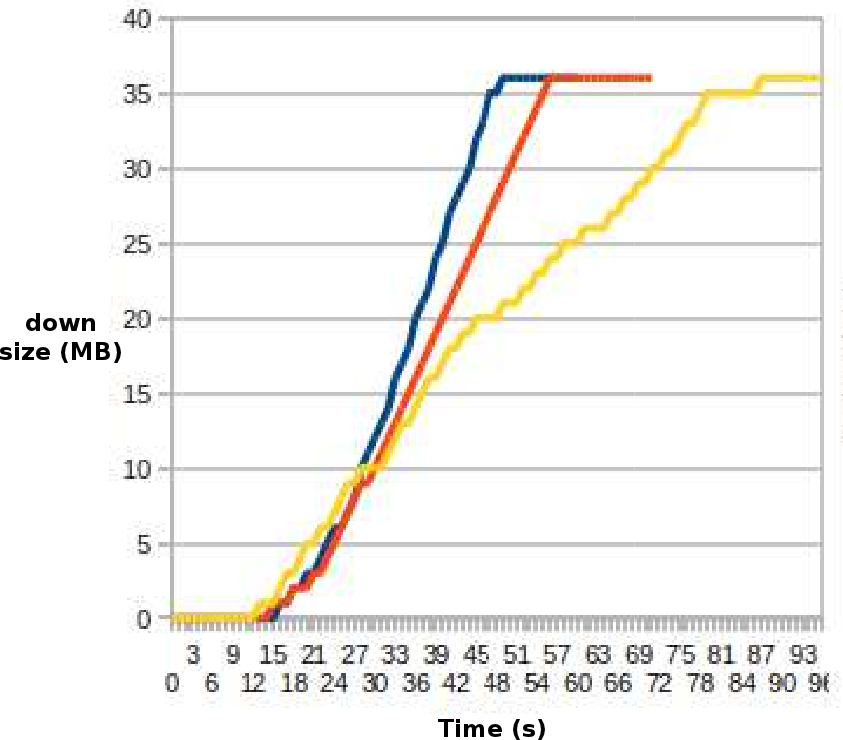
\includegraphics[width=0.35\textwidth]{src/img/multimedia-dist/libtorrent-down-size}
  \label{fig:multimedia-dist:libtorrent-down-size}
  }
%  \subfloat[Download Speed Evolution]{
  \subfloat[Evoluția vitezei]{
  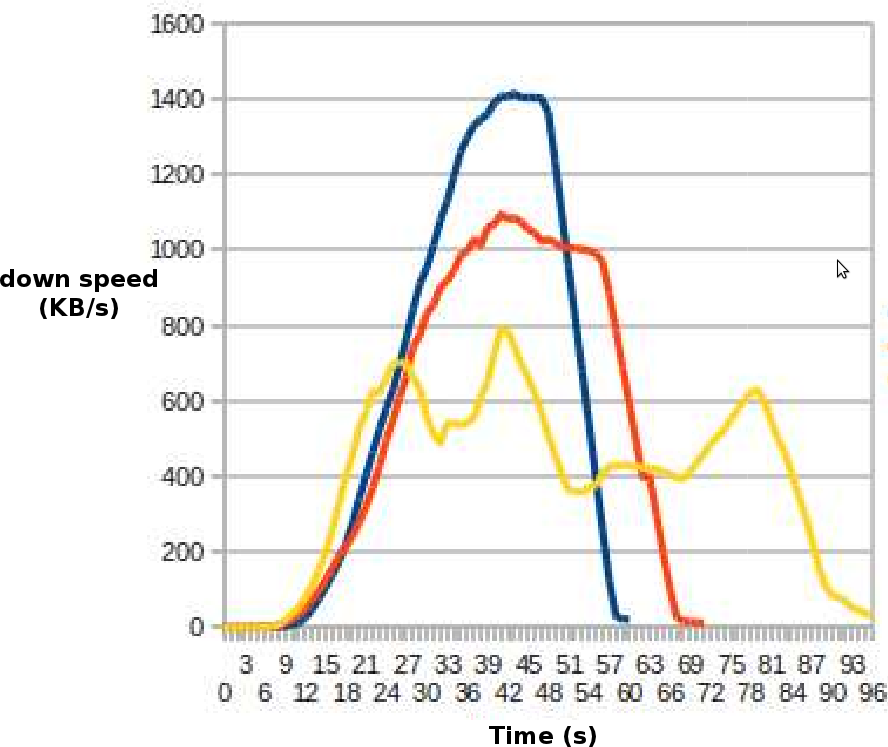
\includegraphics[width=0.35\textwidth]{src/img/multimedia-dist/libtorrent-down-speed}
  \label{fig:multimedia-dist:libtorrent-down-speed}
  }
%  \caption{Evolution of Different Piece Selection Policies}
  \caption{Evoluția diferitor politici de selecție a fragmentelor}
  \label{fig:multimedia-dist:libtorrent-evolution}
\end{figure}

% During this experiment, the best algorithm was, as expected, the
% \textit{rarest first}. We estimate the \textit{deadline piece} was
% outperformed by the \textit{sequential} algorithm, due to the file size being
% quite small, a large number of seeders and the implementation overhead of the
% former for a relatively small file.
În cadrul acestui experiment, ce mai bun algoritm a fost, după cum era de
așteptat, cel care urmează strategia \textit{rarest first}. Se estimează că
algoritmul \textit{deadline piece} a fost depășit de algoritmul
\textit{secvențial} datorită dimensiunii destul de mici a fișierului,
numărului mare de clienți ce puneau la dispoziție datele și datorită
penalizării induse de implementarea primul algoritm pentru fișiere
relativ mici.

% \section{Using NextShare Technology for P2P Streaming}
\section{Folosirea tehnologiei NextShare pentru redare P2P}
\label{sec:multimedia-dist:nextshare}

% The P2P-Next project was started in 2008 as an EU FP7 project. It aims at
% delivering the next-generation Peer-to-Peer content delivery platform. The
% project takes into account the change in the audio video media landscape, with
% increased demand for content availability on the Internet and user participation
% in generation of content. P2P-Next takes into account existing challenges such
% as legal frameworks and business constraints to create a viable solution with
% widespread adoption.
Proiectul P2P-Next a fost început în 2008 ca un proiect EU FP7. Are ca obiectiv
livrarea următoarei generații de platforme Peer-to-Peer pentru distribuția de
conținut. Proiectul ia în considerarea schimbările ce au avut loc în zona
conținutului audio video, cu o creștere a cererii pentru conținutul disponibil
pe Internet și cu implicare a utilizatorilor în generarea de conținut.
P2P-Next ia de asemnea în considerare provocări cu privire la cadrul legal și
constrângeri legate de mediul de afaceri pentru a crea o soluție viabilă,
adoptată pe scară largă.

% Intelligence, resource management, and explicit memory are the foundations for
% the P2P-Next content sharing platform called: NextShare. The NextShare
% system is a self-organizing system with complete decentralisation and hence
% lacks any central bottleneck or choke points that may hamper performance,
% induce setup cost, or require maintenance. Networking effects ensure that
% content, communities, communication, and commerce will flourish with more
% participants.
Inteligența, managementul resurselor și memoria explicită sunt fundația pentru
platforma pentru distribuție de conținut P2P-Next numită NextShare. Sistemul
NextShare este un sistem cu auto-organizare complet descentralizat și, prin
urmare, lipsit de puncte de strangulare ce ar putea altera preformanța, ar
putea induce costuri de configurare sau ar putea necesita întreținere.
Rețeaua asigură ca atât conțintul, cât și comunitățile, comunicarea și
comerțul se vor bucura de mai mulți participanți.

% NextShare is a complex architecture integrating features that are common to
% BitTorrrent applications but also those integrating streaming content.
NextShare are o arhitectură complexă ce integrează trăsături caracteristice
aplicațiilor de BitTorrent, precum și trăsături caracteristice aplicaților de
redare de conținut.

% NextSharePC runs on PC, supporting Windows, Linux and MacOS X Operating
% Systems/distributions. NextSharePC application is formed by two parts:
% \begin{itemize}
%   \item A back-end server called NextShare Agent (NSSA), which embeds the P2P
%   core engine (NextShareCore).
%   \item A front-end part in charge of providing the user interface and content
%   playback functionalities.
% \end{itemize}
NextSharePC rulează pe PC, oferind suport pentru sistemele de
operare/distribuțiile Windows, Linux și MacOS X. Aplicația NextSharePC este
formată din două părți:
\begin{itemize}
  \item Un server back-end numit NextShare Agent (NSSA) ce cuprinde motorul
  central P2P (NextShareCore)
  \item O parte de front-end responsabilă pentru oferirea interfeței grafice
  și capabilităților de redare a conținutului
\end{itemize}

% The split between front-end and back-end let the P2P engine (NSSA) run in the
% background regardless if the front-end interface (GUI) is running or not. This
% enables the peer to share content within the NextShare network even if the
% user is not in front of the PC and/or is not interacting with NextSharePC.
Delimitarea dintre front-end și back-end permite motorului P2P (NSSA) să
ruleze în fundal indiferent dacă interfața front-ent (GUI) rulează sau nu. 
Acest lucru permite clientului să distribuie conținut în cadrul rețelei
NextShare chiar și dacă utilizatorul nu se află în fața PC-ului și/sau nu
interacționează cu NextSharePC.

% Initially an improved BitTorrent core aiming for improved performance and
% diverse features, the NextShare core integrated streaming support. This has
% been mostly due to Jan David Mol's
% work~\cite{give-to-get}~\cite{design-p2p-live} in getting streaming
% support in NextShare. Currently, NextShare supports both Video-on-Demand
% and live streaming. Both stream features are enabled through the use of
% mesh-like overlays, regarded as swarm topologies, due to their working on top
% of BitTorrent.
Pornit inițial ca o versiune îmbunătățită a nucleului BitTorrent cu obiectivul
de a crește performanța și a diversifica opțiunile oferite, nucleul NextShare
a integrat suportul pentru redarea de conținut media. Acest lucru se datorează
în cea mai mare parte muncii lui Jan David Mol
~\cite{give-to-get}~\cite{design-p2p-live} pentru adăugarea de suport pentru
redare în NextShare. În prezent, NextShare oferă suport atât pentru
Video-on-Demand și redare în timp real. Ambele opțiuni pentru redare sunt
activate prin folosirea unor suprapuneri sub formă de rețea, privite ca
topologii de grup, datorită modalității de funcționare peste BitTorrent.

% VoD support in NextShare is enabled through the deployment of Give-to-Get, a
% novel approach to negotiating piece exchange. Give-to-Get features many
% similarities to BitTorrent's own tit-for-tat protocol, but differs in certain
% areas which make it more suitable for video-on-demand. Specifically, while in
% offline download mode (classical distribution), the tit-for-tat protocol marks
% a peer's ``altruism'' by its history, Give-to-Get only checks its recent
% history. In VoD, a peer is interested in exchanging information from peers that
% can offer him current pieces, in order to sustain video playback; if a peer
% has been altruistic with early pieces if of little relevance to the current
% peer.
Suportul pentru VoD în NextShare este activat prin implementarea Give-to-Get,
o nouă abordare pentru negocierea schimbului de fragmente. Give-to-Get prezintă
multe asemănări cu protocolul tit-for-tat propriu BitTorrent, dar diferă în anumite
aspecte ce îl fac mai potrivit pentru Video-on-Demand. Mai specific, cât timp se
află în modul de descărcare offline (distribuție clasică), protocolul tit-for-tat
marchează ,,altruismul'' unui client în funcție de istoria acestuia, în timp ce
Give-to-Get verifică doar istoria recentă.

% While most implementation use a tree-based or multi-tree based approach for
% live streaming, NextShare's BitTorrent core required a swarm-based approach.
% Each peer will connect to a given set of peer and request pieces from those.
% Major updates had to be undertaken due to the differences between offline
% playback (classical distribution) and live streaming: the size of the file is
% unknown, there is no seeder, there are no hashes for integrity checking,
% pieces have to be retrieved real time. This required careful updates to the
% piece picking component of the BitTorrent engine and the selection of peers in
% the neighbor set.
În timp ce majoritatea implementărilor folosesc o abordare bazată pe un arbore
sau multi-arbore pentru redarea live, nucleul BitTorrent al lui NextShare
are nevoie de o abordare bazată pe grupuri. Fiecare client se va conecta la
un anumit set de clienți și va cere fragmente de la aceștia. Actualizări
majore au trebuit întreprinse datorită diferențelor dintre redarea offline
(distribuție clasică) și redarea live: dimensiunea fișierului este necunoscută,
nu există un distribuitor, nu există hash-uri pentru verificarea integrității,
fragmentele trebuie obțiune în timp real. Aceasta a necesitat actualizări
atente ale componentelor de selecție a fragmentului a motorului BitTorrent și
de selecție a clienților în setul de vecini.

% The LivingLab is the mechanism by which NextShare based application get
% tested ``in the while'' i.e. with real users and real environments. In the
% P2P-Next project the LivingLabs are located in several partner locations such
% as Lancaster (UK), Tromso (Norway), Tampere (Finland), Ljubljana (Slovenia)
% and Bucharest (Romania).
LivingLab este mecanismul prin care aplicațiile bazate pe NextShare sunt
testate de utilizatori reali, în medii de lucru reale. În proiectul P2P-Next,
grupurile LivingLab sunt localizate în mai multe locații partenere, cum ar fi
Lancaster (Norvegia), Tampere (Finlanda), Ljubljana (Slovenia) și București
(România).


% The UPB LivingLab consists of several commodity hardware systems kindly
% provided by the NCIT cluster. These systems store content used for the
% LivingLab and the applications, scripts and services that power it. All
% systems are identical both from a hardware perspective and by means of
% software applications and content.
Grupul LivingLab din UPB constă din mai multe sisteme hardware puse la
dispoziție prin amabilitatea clusterului NCIT. Aceste sisteme stochează
conținutul folosit de LivingLab, precum și aplicațiile, scripturile și
serviciile care îl fac posibil. Toate sistemele sunt identice atât din
perspectiva hardware-ului folosit, cât și din prizma aplicațiilor și a
conținutului.

% The LivingLab site, described in detail in
% Section~\ref{subsec:multimedia-dist:evaluation-infrastructure} provides the
% interface with the help of which users access content using NextShare
% technology. It possess a large number of VoD assets from various events that
% are available to be played back using the SwarmPlugin. Assets are HD content
% in MP4 and OGG container format. The LivingLab describes useful information to
% users and provides a forum where questions may be asked and support may be
% requested.
Pagina LivingLab pune la
dispoziție interfața prin are utilizatorii accesează conținutul folosind
tehnologia NextShare. Aici se poate găsi un număr mare de obiecte VoD de la
diverse evenimente, disponibile pentru redare folosind SwarmPlugin. Obiectele
sunt continut HD în format MP4 și OGG. LivingLab oferă utilizatorului informații
utile și pune la dispoziție un forum unde se pot pune întrebări și se poate
cere suport.

% Various experiments have taken place in the UPB LivingLab, the most recent
% ones being described in Section~\ref{sec:multimedia-dist:evaluation}. As the
% UPB LivingLab is focused on performance management and analysis, experiments
% were keen on measuring BitTorrent swarm information and gathering relevant
% information.
% The current and overall goal of the trials to be deployed and the UPB
% LivingLab is comparing Peer-to-Peer streaming performance and functionalities
% to classical distribution. We aim to collect relevant internal information
% regarding the behavior of the technology both when used for VoD streaming and
% for BitTorrent swarm download and use that information for signaling points
% that should be taken into account to improve streaming performance, mostly
% related to peer download speed.
Diverse experimente au fost conduse în cadrul LivingLab din UPB, cele mai
recente fiind descrise în Secțiunea~\ref{sec:multimedia-dist:evaluation}.
Deoarece LivingLab din UPB se concentrează pe managementul performanței și
analiză, experimentele și-au dorit să măsoare date despre grupurile
BitTorrent și despre acumularea informației relevante.
Scopul actual și global al acestor încercări ce for fi desfășurate și al
grupului LivingLab din UPB este compararea performanței redării și a
funcționalităților Peer-to-Peer cu distribuția clasică. Urmărim să colectăm
informație internă relevantă cu privire la modul de comportare al tehnologiei
atât atunci când este folosită pentru redare VoD, cât și în cadrul grupurilor
BitTorrent și să folosim această informație pentru semnalarea aspectelor
care ar trebui luate în considerare pentru îmbunătățirea performanței redării,
aspecte legate în cea mai mare parte de viteza de descărcare.


% \section{Evaluation of P2P Streaming Solutions}
\section{Evaluarea soluțiilor de streaming P2P}
\label{sec:multimedia-dist:evaluation}

% Within the UPB LivingLab, experiments that involve users, HD content and the
% NextShare streaming solutions have and are currently taking place. The goal is
% to provide useful information on the functionality of the solution, the user
% experience and transfer performance. As the goal of the P2P-Next project
% is to built the next-generation Peer-to-Peer content delivery platform, our
% aim is to provide useful information regarding key factors that influence its
% attractiveness. Questions such as the ones below need to be answered: Would
% people use this platform instead of
% YouTube? Would it outperform classical video streaming? How does it compare to
% classical BitTorrent distribution performance?
În cadrul LivingLab din UPB, experimente care implică utilizatorii, conținut
HD și soluția NextShare de redare au fost desfășurate și continuă să se
desfășoare și în prezent. Scopul este de a pune la dispoziție informații despre
funcționalitatea soluției, experiența utilizatorilor și performanța transferului.
Cum scopul proiectului P2P-Next este de a construi următoarea generație de
platforme Peer-to-Peer pentru distribuția de conținut, obiectivul nostru este
acela de a obține informații despre factorii cheie care influențează adopția
acestuia. Întrebări ca cele de mai jos trebuie să primească un răspuns:
Ar folosi utilizatorii această platformă în locul YouTube? Va reuși să
depășească performanțele redării video clasice? Cum se comportă din punct de
vedere al performanței distribuției în comparație cu soluția clasică
BitTorrent?

% The UPB LivingLab is the user window to the NextShare technology. It
% provides instructions on using the technology and allows access to the content
% and facilities. From a user's point of view,
% the LivingLab is the site/portal/frontend allowing the playback of various video
% files through the use of P2P technology. In the backend, the LivingLab is
% supported by systems in the NCIT cluster that store and serve content in the
% form of Video-on-Demand assets.
Laboratorul LivingLab din UPB este fereastra utilizatorilor către tehnologia
NextShare. Pune la dispoziție instrucțiuni despre modul de folosire a
tehnologiei și permite accesul la conținut și facilități. Din punctul de
vedere al unui utilizator, LivingLab este o pagină/portal/frontend ce permite
redarea de fișiere video diverse prin folosirea tehnologiei P2P. În backend,
LivingLab este suportat de sisteme din clusterul NCIT care stochează și servesc
conținutul sub forma de produse Video-on-Demand.

% The NCIT cluster systems are commodity hardware systems that provide content
% and seeders. Content is replicated among NCIT cluster systems and is seeded
% through automated NextShare technology applications. There are currently nine
% systems available. The same content assets are found among multiple systems
% such that there would be multiple seeders for each asset. Logging is enabled
% at seeder level for subsequent processing. Swarm trackers may reside on a NCIT
% system or outside of it; as tracker communication is reduced, its placement is
% of little relevance.
Sistemele de clustere NCIT sunt sisteme hardware care pun la dispoziție
conținut și distribuitori. Conținutul este replicat în cadrul sistemelor de
clustere NCIT și este servit automat prin aplicațiile automate ale tehnologiei
NextShare. În prezent există nouă sisteme disponibile. Același conținut se
găsește pe sisteme multiple, astfel încât vor exista mai mulți distribuitori
pentru același produs. Jurnalizarea este activată la nivel de distribuitor
pentru procesări ulterioare. Grupurile de tracker-e pot rezida într-un sistem
NCIT sau în afara acestuia; deoarece comunicația cu tracker-ul este redusă,
poziționarea lui are o relevanță scăzută.

% User feedback is collected through feedback forms that request information
% about user experience, plugins used, issues encountered. Detailed information
% about feedback forms is provided in
% Section~\ref{subsec:multimedia-dist:evaluation-december-2010}. The feedback
% form has been updated from a Google form-based one to one that is fully
% integrated into the site. At the same time, during experiment evolutions,
% questions were added or were discarded.
Feedback-ul utilizatorilor este colectat prin formulare de feedback care cer
informație despre experiența utilizatorilor, plugin-urile folosite,
problemele întâmpinate.

% A specialized form of user feedback is user log files. During experiments,
% both from our side and from WP4 team members, we have requested users to
% provide us with logging information for troubleshooting issues. As such, we
% have integrated a log upload facility where users can upload basic upload
% information provided by NextShare. Log files are typically no greater than
% 100K, such that there is little overhead or burden in uploading them.
O formă specializată de feedback de la utilizatori este folosirea fișierelor
de jurnalizare ale acestora. În timpul experimentelor, atât cele conduse de
noi, cât și cele conduse de membri ai echipei WP4, utilizatorilor li s-a cerut
să pună la dispoziție informația jurnalizată pentru rezolvarea problemelor.
Prin urmare, a fost integrată o facilitate pentru încărcarea jurnalelor, unde
utilizatorii pot încărca informația jurnalizată de bază ce este pusă la
dispoziție de NextShare.  Fișierele de tip jurnal nu sunt de obicei mai mari de
100K, astfel încât experiența nu este încetinită sau îngreunată prin
încărcarea lor.

% We evaluate streaming performance of NextShare technology through experimental
% means. Trials are setup in the LivingLab and use those to collect logging
% information and use that for analysis and advice. Providing advice regarding
% performance of streaming implementation is the prime concern of our
% evaluation.
Performanța tehnologiei NextShare este evaluată prin mijloace experimentale.
Studiile sunt create în LivingLab, unde se colectează informația jurnalizată și o
folosesc pentru analiză și sfaturi. Punerea la dipoziție de sfaturi cu privire
la performanța implementării redării este prima grijă în cadrul evaluării.

% We use status information such as peer download speed, peer upload
% speed, number of connections and extensive information (usually provided
% through verbose logging) such as protocol messages, protocol inner workings,
% piece picker algorithm (piece selection) to compare and analyze classical
% (pure BitTorrent-based data distribution) to video streaming (through
% NextShare technology). We aim to distinguish among the various patterns
% employed by each type of distribution, measuring variation/penalty in
% performance and identify weak and strong spots in each of the approaches.
Se folosesc informații legate de stare, cum ar fi viteza de descărcare și
încărcare a clienților, numărul de conexiuni, și informație amplă
(obținută de obicei prin jurnalizarea intensă), cum ar fi mesajele din cadrul
protocolului, funcționarea internă a protocolului, algoritmul de selecție
a fragmentului, pentru a compara și analiza soluția clasică
(distribuție de date bazată în totalitate pe BitTorrent) cu soluția cu
redare video (prin tehnologia NextShare). Obiectivul este acela de a 
discerne între diverse tipare impuse de fiecare tip de distribuție,
măsurând variația/penalizările în performanță și identificând punctele
slabe și puternice în fiecare dintre abordări.

% During December we have undertaken a
% medium-sized experiment for evaluating the NextShare technology and user
% satisfaction. The LivingLab site was the center of the experiment: it
% provided the interface for download the NextShare plugin, linking video files,
% publishing the feedback form and providing support through the forum.
În decembrie, am condus un experiment de mărime medie pentru a evalua
tehnologia NextShare și satisfacția utilizatorilor. Pagina LivingLab a fost
centrul experimentului: a pus la dispoziție interfața pentru descărcarea
plugin-ului NextShare, legături către fișierele video, formularul de feedback
și suportul necesar prin forum.

% A total number of 55 users completed the feedback form. A brief of the
% results:
% \begin{itemize}
%   \item users had problems installing the plugin and most of them were
%   unable to properly start the playback;
%   \item video playback was deemed mediocre; some may
%   be due to the problems in installing the plugin;
%   \item the plugin interface was considered to be usable - content playback
%   could be easily enabled;
%   \item most users used the Firefox version of the Plugin;
%   \item users were using high bandwidth connections ($>$ 512KB/s) or fairly
%   good ones ($>$ 50KB/s, $<$ 100KB/s);
%   \item video freezing and the lack of a seek and volume bar were among the
%   most significant remarks.
% \end{itemize}
În total, un număr de 55 de utilizatori au completat formularul de feedback.
Un sumar al rezultatelor:
\begin{itemize}
  \item utilizatorii au întâlnit probleme în instalarea plugin-ului și cei mai
  mulți dintre ei s-au aflat în incapacitatea de a porni redarea;
  \item redarea video a fost considerată mediocră; o parte din aceste considerente
  pot fi legate de problemele întâmpinate în instalarea plugin-ului;
  \item interfața plugin-ului a fost considerată utilizabilă - redarea conținutului
  a putut fi ușor activată;
  \item cei mai mulți dintre utilizatori au folosit versiunea Firefox a plugin-ului;
  \item utilizatorii au folosit conexiuni cu lățime de bandă ridicată ($>$ 512KB/s)
  sau cu lățime de bandă destul de bună ($>$ 50KB/s, $<$ 100KB/s);
  \item oprirea bruscă a redării și lipsa unui control pentru volum și progres s-au
  aflat printre cele mai semnificative remarci.
\end{itemize}

% The April 2011 Experiment was focused on testing basic functionality for
% comparison between classical distribution versus streaming. The aim is to set
% up all pieces required for experimentation, data collection and analysis. In
% order to accomplish this data was collected both from classical BitTorrent
% clients such as uTorrent, Transmission and streaming functionality. Users were
% instructed to use both the NextSharePC plugin and a classical distribution
% BitTorrent client in order to provide information required for comparison.
Experimentul din aprilie 2011 s-a concentrat pe testarea funcționalității de
bază pentru a compara distrbuția clasică cu redarea. Obiectivul este de a
pune la punct toate piesele necesare pentru experimentare, colectarea de date
și analiză. Pentru a atinge acest obiectiv, datele au fost colectate atât de la
clienți clasici BitTorrent, cum ar fi uTorrent, Transmission, cât și din
produsul cu funcționalitate de streaming. Utilizatorii au fost instruiți să
folosească atât plugin-ul NextSharePC, cât și un client pentru distribuție
clasică BitTorrent pentru a putea pune la dispoziție informațiile necesare
pentru comparație.

% Logging had been enabled at seeder level. Due to the high level of information
% only status information such as download speed, upload speed, peer connections
% had been collected in log files. A high quantity of data was collected
% resulting in 100GB of status log information per seeder in two months time. In
% order to match IP information from seeder logs to BitTorrent clients, logging
% had also been enabled at tracker level. Tracker log files display global
% information regarding swarms and periodic information (typically once every 30
% seconds) from announce messages from clients.
Logarea a fost activată la nivel de distribuitor. Datorită cantității ridicate de
informație, doar informație de stare precum viteza de descărcare și încărcare,
conexiunile cu alți clienți au fost colectate în fișierele jurnal. O contitate
ridicată de date a fost colectată, rezultând în 100GB de informația jurnalizat de stare
per distribuitor într-un interval de două luni. Pentru a putea face o corespondență
între informația IP din fișierele jurnal ale distribuitorului și clienții BitTorrent,
jurnalizarea a fost activată, de asemenea, la nivel de tracker. Fișierele
jurnal pentru
tracker-e afișează informație globală cu privire la grupuri și informație periodică
(în mod tipic o dată la 30 de secunde) în legătură cu mesajele de anunț primite de
la clienți.

% Important updates had been implemented since the December experiment, based on
% user feedback and updated goals. VLC-based API for playback interaction (such
% as a progress bar, volume selection, pause, resume) had been added.
Actualizări importante au fost implementate de la experimentul din decembrie,
bazate pe feedback-ul primit de la utilizatori și pe noile obiective. Un API de tip
VLC pentru interacțiunea cu redarea (cum ar fi un control pentru progres, selecția
volumului, pauză sau continuare) a fost adăugat.

% Apart from the VLC-based NextSharePC plugin, the site was added the
% Firefox-based plugin using HTML5 technology. Thus, for each VoD assed, there
% would be two types of files: MP4+H.264 for the VLC-based plugin and OGG+Theora
% for the HTML5-based plugin. Users were provided with links to the other
% version of the file. This allowed using NextShare technology on Linux-based
% systems.
Pe lângă plugin-ul NextSharePC de tip VLC, paginii i-a fost adăugat și un plugin
pentru Firefox ce folosește tehnologia HTML5. Prin urmare, pentru fiecare
produs VoD, există două tipuri de fișiere: MP4+H.264 pentru plugin-ul bazat pe
VLC și OGG+Theora pentru plugin-ul bazat pe HTML5. Utilizatorilor le-au fost
puse la dispoziție adrese și către celelalte versiuni ale fișierelor. Aceasta
a permis folosirea tehnologiei NextShare și pe sisteme bazate pe Linux.

% There were several updates to the site and user interaction, also as part of
% user plugin or suggestions from inside the P2P-Next WP4 or WP8 teams. The log
% file upload form had been changed from a rather user-unfriendly FTP-based form
% to one based on HTTP. The feedback form had also been updated to discard
% information that could be retained otherwise (from browser information, for
% example – the IP address, operating system, browser, or from BitTorrent client
% provided information – average download/upload speed).
De asemenea, au fost realizate mai multe actualizări ale paginii și ale
interacțiunii cu utilizatorii, ca urmare a plugin-ului pentru utilizatori sau
ale sugestiilor venite din interior din partea echipelor P2P-Next WP4 sau WP8.
Formularul pentru încărcarea fișierului jurnal a fost schimbat de la un formular
destul de neprietenos bazat pe FTP la unul bazat pe HTTP. De asemenea, formularul
de feedback a fost actualizat pentru a renunța la informația care putea fi obținută
pe alte căi (din cadrul browser-ului, de exemplu - adresa IP, sistemul de operare,
browser-ul, sau din informația pusă la dispoziție de clientul de BitTorrent -
viteză medie pentru descărcare/încărcare).

% 42 users had correctly presented their IP addresses. Users had found the
% plugin and technology fun to use and provide feedback, both from an average
% user's perspective and from a technical user's perspective. Features that have
% been praised were:
% \begin{itemize}
%   \item Fast download speed.
%   \item Easy installation.
%   \item Good video quality.
% \end{itemize}
Un număr de 42 de utilizatori au oferit în mod corect adresele lor IP. Utilizatorii
au considerat plugin-ul și tehnologia distractiv de folosit și au oferit feedback,
atât din puctul de vedere al unui utilizator mediu, cât și din punctul de vedere al
unui utilizator cu cunoștințe tehnice. Caracteristicile care au fost apreciate
au fost viteza mare pentru descărcare, instalarea facilă, calitatea video bună.

% The important issues had been tackled after the trial, some of them being
% described in detail in Section~\ref{subsec:multimedia-dist:evaluation-issues}.
% The most stringent issue deals with
% playback problems in the NextShare player for a diversity of video files. This
% was due to multiple reasons. One of them of the absence of a bitrate
% information in the .torrent/.tstream file; the client was unable to properly
% render the video. Another cause was the 
Problemele importante au fost abordate după studiu.  Cele mai stringente
probleme sunt cele legate de problemele la redarea video în player-ul
NextShare pentru o diversitate de fișiere video. Aceasta s-a datorat mai
multor motive. Unul dintre ele a fost absența informației despre bitrate în
fișierul .torrent/.tstream; clientul s-a aflat în incapacitatea de a reda
corect fișierul video.

% As mentioned, users were requested to use dual clients to provide sample
% information from classical BitTorrent distribution clients and from the
% NextSharePC plugin as a representative of P2P streaming solutions. Download
% and upload rate for the NextSharePC is limited to 1MB/s for performance
% consideration such that preliminary results have little relevance other than
% providing sample information and testing the existing infrastructure.
După cum a fost menționat, în cadrul experimentului din aprilie 2011, utilizatorilor li s-a cerut să folosească în mod dual
clienții pentru a pune la dipoziție informație despre distribuția clasică
BitTorrent și despre plugin-ul NextSharePC, ca reprezentat la soluțiilor de
redare P2P. Rate de descărcare și încărcare pentru NextSharePC este limitată
la 1MB/s din considerente de performanță, astfel încât rezultatele preliminare
au relevanță scăzută în afara scopului de a oferi probe și de a testa
infrastructura existentă.

% Sample results were:

% \begin{itemize}
%   \item ``classical'' clients used (no recommendation was given to users)
%   were: uTorrent (16), Transmission (9) and BitTorrent mainline (2)
%   \item NextSharePC download speed varied between 300KB/s and 800KB/s
%   \item Transmission download speed: 500KB/s-1500KB/s
%   \item uTorrent download speed: 1000KB/s-4000KB/s
% \end{itemize}
Rezultatele obținute:
\begin{itemize}
  \item clienți clasici folosiți (utilizatorii nu au primit o recomandare)
  au fost: uTorrent (16), Transmission (9) și ramura principală a BitTorrent (2)
  \item viteza de descărcare pentru NextShare a variat între 300KB/s și 800KB/s
  \item viteza de descărcare pentru Transmission: 500KB/s-1500KB/s
  \item viteza de descărcare pentru uTorrent: 1000KB/s-4000KB/s
\end{itemize}

% Figure~\ref{fig:multimedia-dist:ds-evolution-full} represents the download
% speed by client types during a wider window of the April 2011 trial.
% Figure~\ref{fig:multimedia-dist:ds-evolution-day} uses a smaller window
% centered around a time interval that provided a high number of client
% connections (between 8:00PM and 11:00PM on April 13, 2011). Each client type
% uses a specific color in the figure. As noticed, the NextSharePC client is
% limited to 1MB/s, while Transmission and uTorrent usually perform better. As
% users were requested to use NextSharePC and another client, the NextSharePC
% client is responsible for a large chunk of the plot.
Figura~\ref{fig:multimedia-dist:ds-evolution-full} prezintă viteza de descărcare
în funcție de tipul de client folosit într-un cadru mai larg din timpul studiilor
din aprilie 2011. Figura~\ref{fig:multimedia-dist:ds-evolution-day} folosește
o fereastră mai mică, centrată în jurul unui interval de timp în care a existat
un număr mare de clienți conectați (între 8:00PM și 11:00PM pe 13 aprilie, 2011).
Fiecare tip de client este reprezentat cu o culoare specifică în figură. După cum
se remarcă, clientul NextSharePC a fost limitat la 1MB/s, în timp ce Transmission
și uTorrent se comportă de obicei mai bine.

\begin{figure}
  \centering
  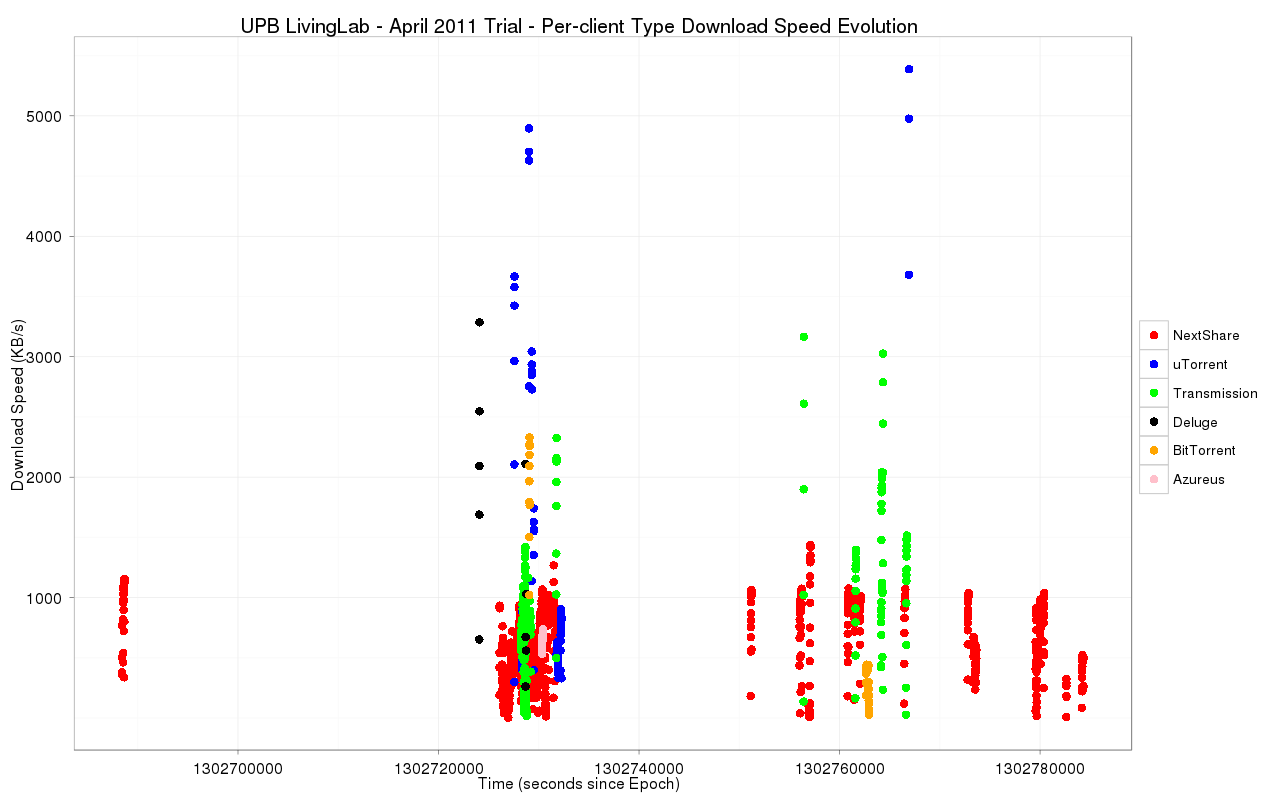
\includegraphics[width=0.6\textwidth]{src/img/multimedia-dist/ds-evolution-full}
%  \caption{April Trial -- Download Speed Evolution by Client Type}
  \caption{Studiul din aprilie -- Evoluția vitezei de descărcare în funcție de
	  tipul clientului}
  \label{fig:multimedia-dist:ds-evolution-full}
\end{figure}

\begin{figure}
  \centering
  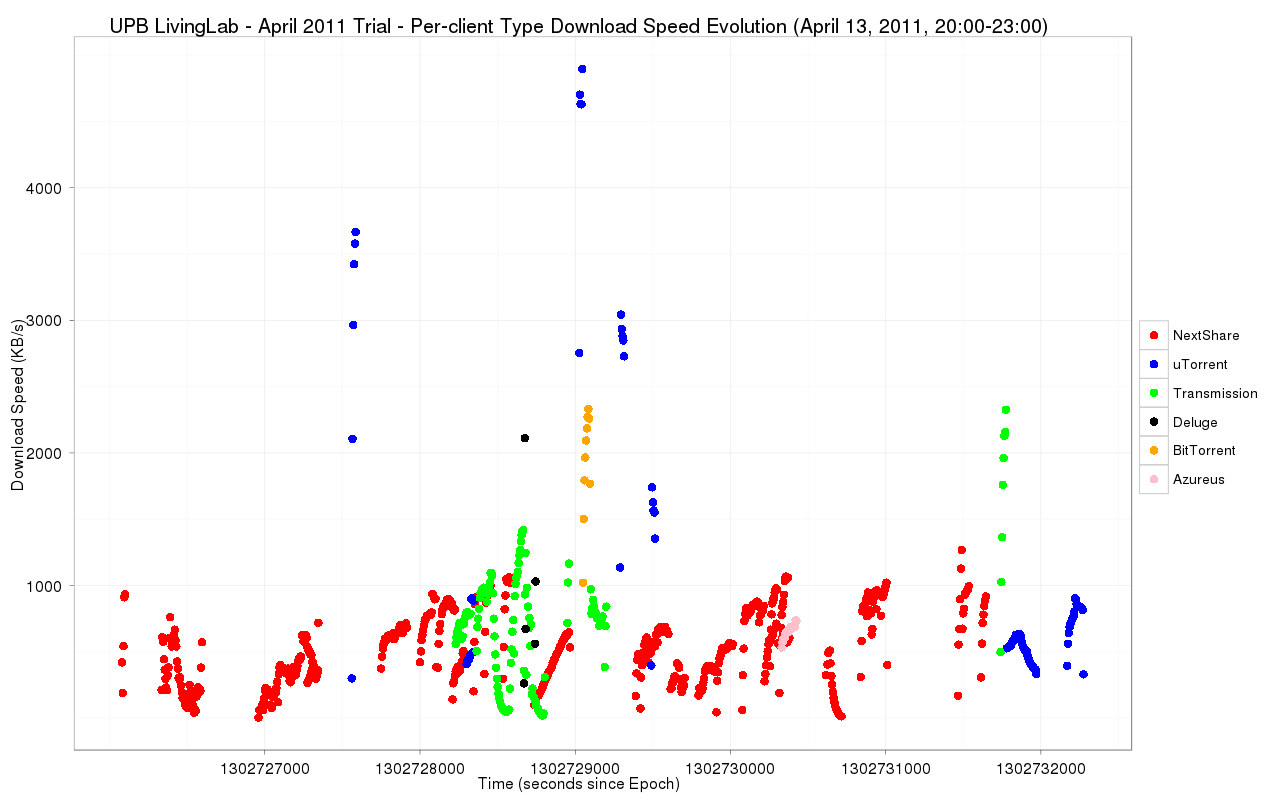
\includegraphics[width=0.6\textwidth]{src/img/multimedia-dist/ds-evolution-day}
%   \caption{April Trial -- Download Speed Evolution by Client Type
%   (8:00PM-11:PM, April 13, 2011)}
  \caption{Studiul din aprilie -- Evoluția vitezei de descărcare în funcție de
	  tipul clientului (8:00PM-11:00PM, 13 aprilie, 2011)}
  \label{fig:multimedia-dist:ds-evolution-day}
\end{figure}
